\documentclass[12pt]{article}

\usepackage[spanish]{babel}
\usepackage[utf8]{inputenc}
\usepackage{graphicx}
\usepackage{geometry}
\usepackage{xcolor}
\usepackage{fancyhdr}
\usepackage{lastpage}
\usepackage{pdfpages}
\usepackage{listings}
\usepackage{schemata}

\geometry{top=25mm,left=15mm,right=15mm,a4paper}

\pagestyle{fancy}
\fancyhf{}
\lhead{Redes de Computadoras}
\cfoot{Página \thepage\ de \pageref{LastPage}}

\graphicspath{./}

\begin{document}
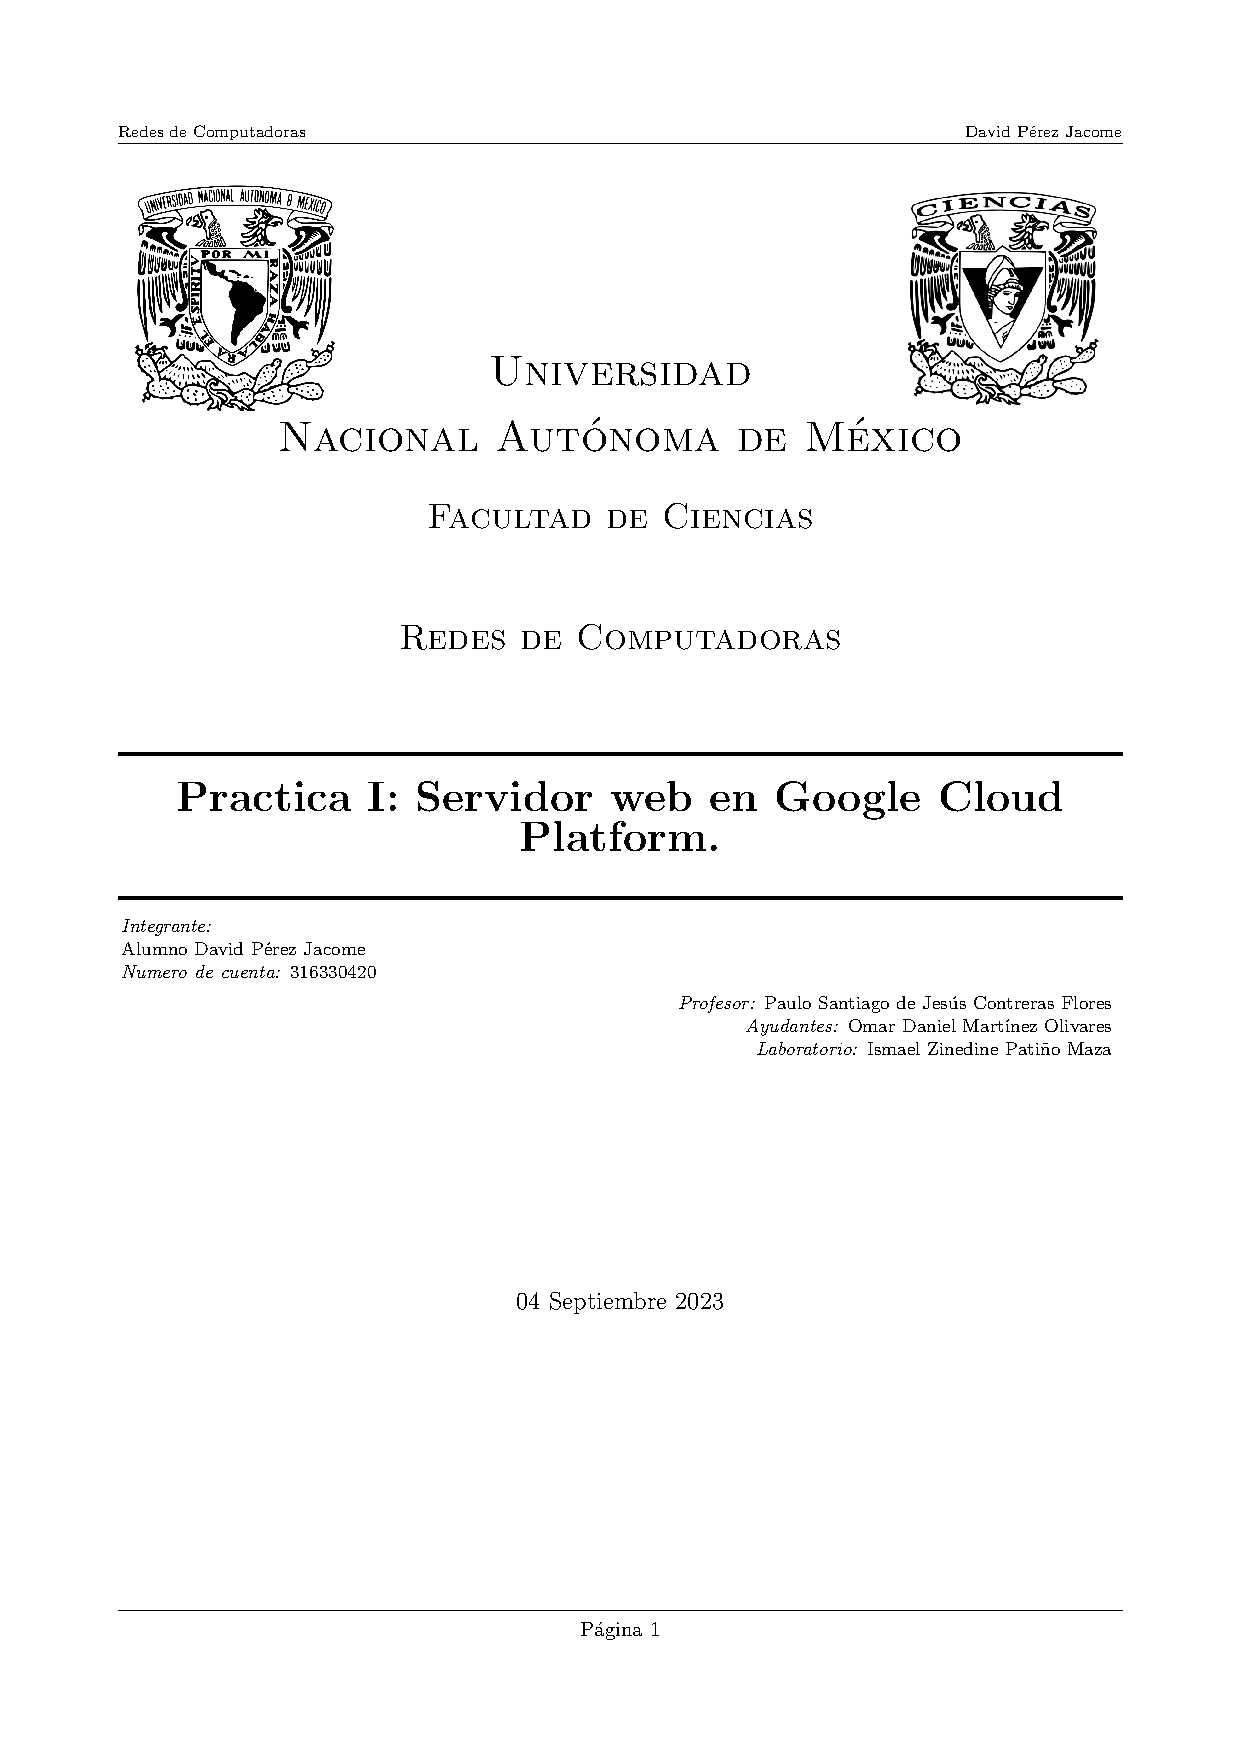
\includepdf{Portada.pdf}
{\color{red} \section*{\textbf{Practica I: Servidor web en Google Cloud Platform..}}}
\vspace{1em}

{\color{blue} \subsection*{\textbf{Objetivo.}}}
\vspace{1em}
El alumno instalará el servidor web Apache HTTPD, y publicará un formulario HTML en este servidor. Además, se familiarizará con el uso de los servicios GCP, VM Instances, Firewall Rules y Static public IP, proporcionados por Google Cloud.
\vspace{2em}

{\color{blue} \subsection*{\textbf{Introducción.}}}
\vspace{1em}
El protocolo HTTPS (HyperText Transfer Protocol Secure) es un protocolo de la Capa de aplicación que permite el envió de información cifrada usando los protocolos HTTP y SSL/TLS. El protocolo HTTP envía información en claro a través del medio, el protocolo SSL/TLS es el encargado de encapsular el protocolo HTTP para ser enviado de manera cifrada.
\vspace{2em}


{\color{blue} \subsection*{\textbf{Desarrollo.}}}
\vspace{1em}
\begin{enumerate}
    \item Creación de cuenta en google cloud.
    \item Creación y configuración de instacia.
    \item Conexión por SSH via web.
    \item Instalación del servidor Apache.
    \item Creación y asignación de reglas de firewall.
    \item Asiganación de IP publica fija.
    \item Visualización web.
    \item Asignación de un formulario web.
\end{enumerate}
\vspace{2em}

{\color{blue} \subsection*{\textbf{Evaluación.}}}
\vspace{1em}
\begin{enumerate}
    \item ¿Qué es el concepto de nube y a qué se refiere el término IaaS?
    \item ¿Qué ventajas observas al utilizar la infraestructura que utilizamos en esta práctica?
    \item Colocar comentarios sobre la práctica
\end{enumerate}








\end{document}